\newpage
\subsection{MapReduce Algorithmus}
MapReduce ist ein von Google Inc. entwickeltes und eingeführtes Programmiermodell. Es wurde speziell zur nebenläufigen Berechnung über große Datenmengen auf Computerclustern entworfen. MapReduce nutzt dabei mehrere Phasen - Map, Shuffle, Reduce - um die Daten zu verarbeiten. Dabei können zwei der Phasen durch den Anwender parametrisiert werden. So lassen sich die Berechnungen parallelisieren und über mehrere Computer verteilen. In einigen Fällen ist eine Parallelisierung alleine durch die großen Datenmengen unumgänglich, da ein einzelner Prozess mit der Verarbeitung überfordert wäre.\\ MapReduce nutzt dafür eine verteilte Speicherung der Daten in Blöcken. Dies sorgt für Datenqualität bei fehlerhaften Schreib- oder Lesevorgängen. Des Weiteren lässt sich MapReduce mit handelsüblichen Computer verwenden. Es ist keine spezielle Server Hardware nötig.(vgl. \cite{wik15})

\paragraph{Definition der $MapReduce$ Funktion}$\;$ \\
Die $MapReduce$ Funktion baut sich aus zwei separaten Abläufen, $Map$ und $Reduce$, auf. Der Input wird aus einer Menge unstrukturierten oder semi-strukturierten Daten gebildet. Die Basis der $Map$ und $Reduce$ Abläufe ist die Bildung von Schlüssel-Wert-Paaren. Es wird aus einer Liste von Schlüssel-Wert-Paraen eine neue Liste von Schlüssel-Wert-Paaren. Die sich daraus ergebenden Formeln lauten wie folgt:

\begin{center}
    $MapReduce: (K \times V)^\ast \rightarrow (L \times W)^\ast$\\$[(k_1, v_1) \dots ,(k_n, v_n)] \rightarrow [(l_1, w_1) \dots (l_n, w_n)]$
\end{center}
\begin{itemize}
    \item Die Mengen $K$ und $L$ enthalten Schlüssel, die Mengen $V$ und $W$ enthalten Werte.
    \item Alle Schlüssel $k \in K$ sind vom gleichen Typ, z. B. Strings.
    \item Alle Schlüssel $l \in L$ sind vom gleichen Typ, z. B. ganze Zahlen.
    \item Alle Werte $v \in V$ sind vom gleichen Typ, z. B. Atome.
    \item Alle Werte $w \in W$ sind vom gleichen Typ, z. B. Gleitkommazahlen.
    \item Wenn $A$ und $B$ Mengen sind, so ist mit $A\times B$ die Menge aller Paare $(a, b)$ gemeint, wobei $a \in A$ und $b \in B$ (kartesisches Produkt).
    \item Wenn $M$ eine Menge ist, so ist mit $M^*$ die Menge aller endlichen Listen mit Elementen aus $M$ gemeint (angelehnt an den Kleene-Stern) - die Liste kann auch leer sein.
\end{itemize}

Die eigentliche Parametrisierung durch den Nutzer wird durch die beiden Funktionen $Map$ und $Reduce$ ermöglicht.

\begin{center}
    $Map: K \times V \rightarrow (L \times W)^\ast$\\$(k, v) \rightarrow [(l_1, x_1) \dots (l_rk, x_{rk})]$
\end{center}
\begin{center}
    $Reduce: L \times W^\ast \rightarrow X^\ast$\\$(l, [y_1, \dots, y_{sl}]) \rightarrow [w_1, \dots, w_{ml}]$
\end{center}

\paragraph{Map Phase}$\;$ \\
Die Daten sind am Anfang partitioniert und repliziert im Hadoop Cluster. Jeder Rechner liest die lokalen Daten zeilenweise als Schlüssel-Wert-Paare und übergibt sie dem $Map$-Task (Implementation der $Map$ Funktion auf einer Maschine). Der Schlüssel dieser Paare ist meistens der Byte-Offset einer Zeile und der Wert ist die Zeile selbst.Die Ausführung der $Map$ Funktion auf jedes gelesene Paar erzeugt ein anderes temporäres Schlüssel-Wert-Paar. Außerdem sortiert der $Map$-Task seine generierten Paare nach Schlüssel und speichert sie temprär lokal. Es folgt eine Umverteilung der kompletten Ausgaben der Map Phase, indem die temporären Paare mit demselben Key aus allen $Map$-Tasks zum selben $Reduce$-Task gesendet werden.

\paragraph{Shuffle Phase}$\;$ \\
Bevor die Reduce Phase starten kann, müssen die Ergebnisse der Map Phase gruppiert werden anhand ihrer Schlüssel. Dazu ist ein koordinierter Datenaustausch nötig. Die Performance der gesamten $MapReduce$ Funktion hängt maßgeblich von der Geschwindigkeit des Datenaustausch während der Shuffle Phase ab.

\paragraph{Reduce Phase}$\;$ \\
Wurden alle Ergebnisse der Map Phase gruppiert werden die Paare des Zwischenergebnisses an den $Reduce$-Task übergeben. Die $Reduce$ Funktion erzeugt schließlich ein aggregiertes Paar. Wie auch in der Map Phase können in der Reduce Phase die einzelnen $Reduce$-Tasks über mehrere Rechner innerhalb des Clusters verteilt werden.

\begin{figure}
    \centering
    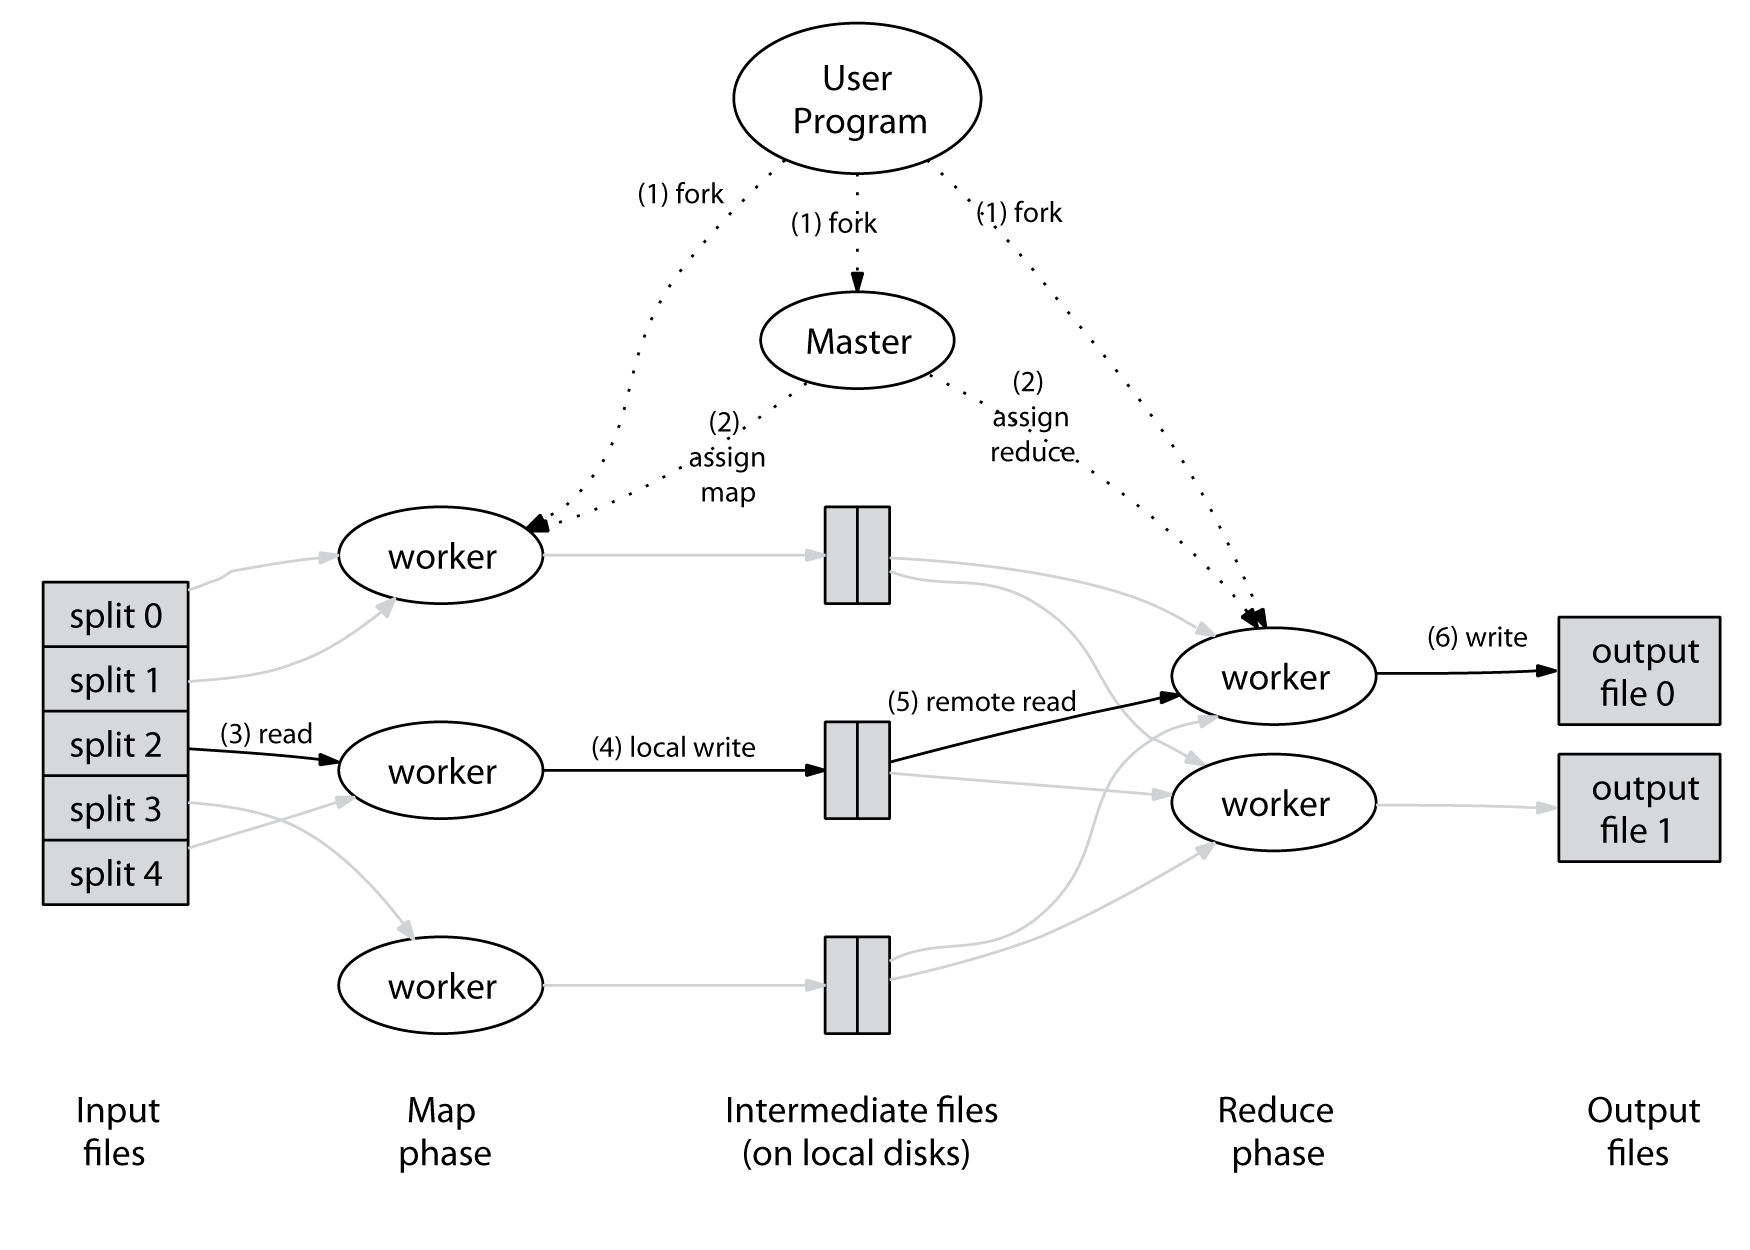
\includegraphics[width=\linewidth]{Mapreduce}
    \caption{Ausführungsreihenfolge von MapReduce\cite{dg04}}
    \label{fig:mapreduce}
\end{figure}

%\paragraph{Beispiel}$\;$ \\
